\chapter{Experiments and Results}
\label{cha:experiments}

Three experiments were conducted in this specialization project. \Autosectionref{sec:experimental-plan-and-setup} will explain how the experiments were conducted, and \autoref{sec:experimental-results} will present the results.

\section{Method: Experimental Plan and Setup}
\label{sec:experimental-plan-and-setup}

\begin{comment}
Trying and failing is a major part of research. However, to have a chance of success you need a plan driving the experimental research, just as you need a plan for your literature search. Further, plans are made to be revised, and this revision ensures that any further decisions made are in line with the work already completed.

The plan should include what experiments or series of experiments are planned and what questions the individual or set of experiments aim to answer. Such questions should be connected to your research questions, so that in the evaluation of your results you can discuss the results wrt to the research questions.

Results should be clearly displayed and should provide a suitable representation of your results for the points you wish to make.
Graphs should be labelled in a legible font. If more than one result is displayed in the same graph, then these should be clearly marked.
Please choose carefully rather than presenting every result. Too much information is hard to read and often hides the key information you wish to present. Make use of statistical methods when presenting results, where possible to strengthen the results.
Further, the format of the presentation of results should be chosen based on what issues in the results you wish to highlight.
You may wish to present a subset in the experimental section and provide additional results in an appendix.
Point out specifics here but save the overall/general discussion to the Discussion chapter.
\end{comment}

The experiments were conducted in order to answer the research questions listed in \autoref{sec:goals-and-research-questions}. As \autoref{sec:gis-with-llms} shows, there have been a substantial body of work on demonstrating the geospatial abilities of \acrshortpl{acr:llm} like ChatGPT, and how these can be used to create larger frameworks for \acrshort{acr:gis} purposes. However, the literature review did not reveal any specific discussions on how \acrshortpl{acr:llm}, like ChatGPT, handle different geospatial file formats, such as \acrshort{acr:gml} or shapefiles, or manage various data access channels. The experiments are designed to address these gaps, with Experiment 1 focusing on \rqref{rq:llm-potential} and ChatGPT's abilities of performing geospatial analysis using different file formats, while Experiment 2 and 3 focus \rqref{rq:overlay-analysis} and \rqref{rq:external-tools} and on its ability to access external web \acrshortpl{acr:api}.

\subsection{Experiment 1: Testing ChatGPT's Ability to Perform Geospatial Data Analysis}

The approach used in Experiment 1 is inspired by the work of \cite{robertsGPT4GEOHowLanguage2023} (see \autoref{sec:gis-with-llms}), who did experiments with increasing difficult on \acrshort{acr:gpt}-4 to characterize what it knows about the geographical world, highlighting both capabilities and limitations. \citeauthor{robertsGPT4GEOHowLanguage2023} focused on \acrshort{acr:gpt}-4's general geospatial awareness, and were not concerned with \acrshort{acr:gis}-related tasks. The reference to \cite{robertsGPT4GEOHowLanguage2023} will therefore be made when highlighting the somewhat surprising geospatial awareness abilities of GPT-4, and the focus of \textit{this} experiment will instead be on displaying its potential for use in the world of \acrshort{acr:gis}. This will be achieved by constructing various tests that aim to reflect \acrshort{acr:gpt}-4's GIS knowledge.

The experiment will utilize the Elveg 2.0 dataset \citep{thenorwegianmappingauthorityElveg2019}, along with cadastral data (including building data, etc.). In order to assess ChatGPT's ability to read and understand different data formats, the data will be provided in \acrshort{acr:sosi}, \acrshort{acr:gml}, GeoJSON, and shapefile formats. Datasets in the first two formats were downloaded from \url{https://geonorge.no}, while the GeoJSON and shapefile datasets were created from the \acrshort{acr:gml} dataset using QGIS. The Elveg 2.0 dataset contains a range of different layers for different types of geometries. In order to simplify the experiments, only the layer named "Fartsgrense" (English: "Speed limit") was used from Elveg 2.0.

Below are the questions that were asked in rising order of predicted complexity:

\begin{enumerate}
    \item \enquote{Provide a summary of the file contents, highlighting the file's most salient features.}
    \item \enquote{Provide a visual representation of the file contents.}
    \item \enquote{Find the mean location of the building locations.}
    \item \enquote{Extract all roads with a speed limit greater than or equal to 80 km/h.}
    \item \enquote{Select all buildings located within 50 metes of a high-speed road (speed limit >= 80 km/h).}
    \item \enquote{Find the area best suited for expansion to accommodate residential buildings.}
\end{enumerate}
\label{enum:gpt-gis-questions}

Some follow-up questions were added when needed, in order help the model understand the questions, or when it stops and asks for permission to go forth with analysis. All conversations are saved in the project's GitHub repository.\footnote{\url{https://github.com/oskarhlm/prosjektoppgave/tree/main/documents/ChatGPT_conversations}}

\subsection{Experiment 2: Comparing File Upload and API Calling in ChatGPT-4}

Another important thing to test is the issue of providing ChatGPT with relevant files on which it can perform analysis. ChatGPT Plus users will have access a range of advanced features, including web browsing with Bing, Dall-E Image Generation, and the Code Interpreter (or Advanced Data Analysis). The latter of these allows the user to manually upload files into the chat instance and perform advanced analyses on the contents of these, which is what was used to upload the datasets in Experiment 1. While this is very powerful, having to manually upload files poses some limitations. A more flexible system should be capable of accessing web \acrshortpl{acr:api} in real time.

A dataset delineating the border of Drammen municipality was utilized to test ChatGPT's capability to analyze manually uploaded data, in comparison to providing it with a URL to an \acrshort{acr:api} endpoint. The data conforms to the GeoJSON standard and contains a FeatureCollection object with a single Feature, namely the border. When the file/\acrshort{acr:api} endpoint had been provided, ChatGPT was simply asked to present a visual presentation of its contents.

The dataset is available through an \acrshort{acr:ogc} \acrshort{acr:api} that was created by Norkart's Alexander Salveson Nossum for testing purposes.\footnote{\url{https://alenos-tester001.azurewebsites.net/}} The \acrshort{acr:api} was deployed using \texttt{pygeoapi},\footnote{\url{https://pygeoapi.io/}} a Python library that implements the \acrshort{acr:ogc} \acrshort{acr:api} standards.

\subsection[Experiment 3: Using ChatGPT's and LangChain to perform API Call]{Experiment 3: Using ChatGPT's and LangChain to perform \acrshort{acr:api} Calls}\label{subsec:ex-3-setup}

A final and third experiment was conducted to see if there are other, more programmatic ways of performing \acrshort{acr:api} calls using \acrshortpl{acr:llm}. The LangChain framework \citep{chaseLangChain2022} was used to create OpenAI functions that can be called using OpenAI's Function calling. The goal of the experiment was to produce the same plot as requested in Experiment 2 using the same \acrshort{acr:api} endpoint.

One function with signature \texttt{make\_http\_request(url: str, save\_file\_name: str)} was made to fetch the data from the \acrshort{acr:api} and save it to a temporary file on the machine from which the code is executed. Another function, \texttt{plot\_geojson(geojson\_path: str)}, was created to load a GeoJSON file from the temporary folder and plot the contents using the Matplotlib library. The hope is that by using LangChain's \texttt{AgentExecutor}, which enables reasoning and chaining responses from an \acrshort{acr:llm}, in conjunction with the Function calling capabilities of the OpenAI \acrshort{acr:gpt} \acrshortpl{acr:api}, should make it possible for the agent to call these functions in the right order and with the correct arguments. The \texttt{gpt-4-1106-preview} model was used for this experiment.

The experiment is only meant to be an initial test to demonstrate how \acrshortpl{acr:llm} can be used to access external tools, thereby supporting \rqref{rq:external-tools}. The current setup is by no means scalable, but is rather meant to demonstrate a technique that can be utilized when developing larger and more capable systems.

\section{Experimental Results}\label{sec:experimental-results}

\subsection{Results for Experiment 1}\label{subsec:experiment-1-results}

\begin{table}
    \centering
    \begin{tabular}{l|p{0.1\textwidth}p{0.15\textwidth}p{0.15\textwidth}p{0.15\textwidth}}
        \toprule
                               & \textbf{\acrshort{acr:sosi}} & \textbf{GML} & \textbf{GeoJSON} & \textbf{Shapefile} \\
        \midrule
        Summary                & No                           & Yes          & Partially        & Partially          \\
        Plotting               & -                            & When guided  & When guided      & Yes                \\
        Mean location          & -                            & When guided  & Yes              & No                 \\
        Filtering              & -                            & No           & Yes              & Yes                \\
        Buffer + Intersect     & -                            & No           & No               & No                 \\
        Planning for expansion & -                            & No           & Partially        & No                 \\
        \bottomrule
    \end{tabular}
    \caption{Overview of the ability of ChatGPT's Code Interpreter to handle various geospatial data formats}
    \label{tbl:data-format-tests}
\end{table}

As \autoref{tbl:data-format-tests} shows, ChatGPT's Code Interpreter is unable to read and write \acrshort{acr:sosi} files. It was unable to manipulate the data directly and was also unable to convert the file into a more suitable format, failing to convert it to GeoJSON using \acrshort{acr:gdal}'s \texttt{ogr2ogr} program. \acrshort{acr:sosi} is therefore excluded from \autoref{tbl:data-format-tests}, which shows the test results on the different file formats.

Furthermore, ChatGPT's Code Interpreter did not manage to properly analyze the \acrshort{acr:gml} data without guidance. It created a parser that was difficult to use for further analysis. When guided into using the GeoPandas library instead---which can handle \acrshort{acr:gml} data---it managed to plot the contents and calculate the centroid of the building points. The \textit{Buffer + Intersect} task \enquote{was interrupted due to its time-consuming nature}, and ChatGPT failed to make an attempt at solving the planning task due to its inability to flexibly analyze the \acrshort{acr:gml} files.

With the GeoJSON data, ChatGPT had difficulties reading the files and could not provide a good summary consistently. It \textit{was} however able to plot the data, but that had to be done in separate responses for each of the two datasets. It was also able to identify the high-speed roads, but could not determine which buildings were located within a 50-meter buffer around these roads. However, when asked to plan for expansion to accommodate residential buildings, it managed to achieve a result close to what was expected in the \textit{Buffer + Intersect} task. It accomplished this by creating a grid and figuring out which grid cells were within 50 meters of a high-speed road. While this did not extract a subset of the building points---which would have been the desired output---it had some minor value in terms of visualization (see \autoref{fig:planning-plot-from-geojson}). Although this result is not particularly useful, it is closer to an acceptable response than the outcomes from the attempts made at the other file formats.

\begin{figure}
    \centering
    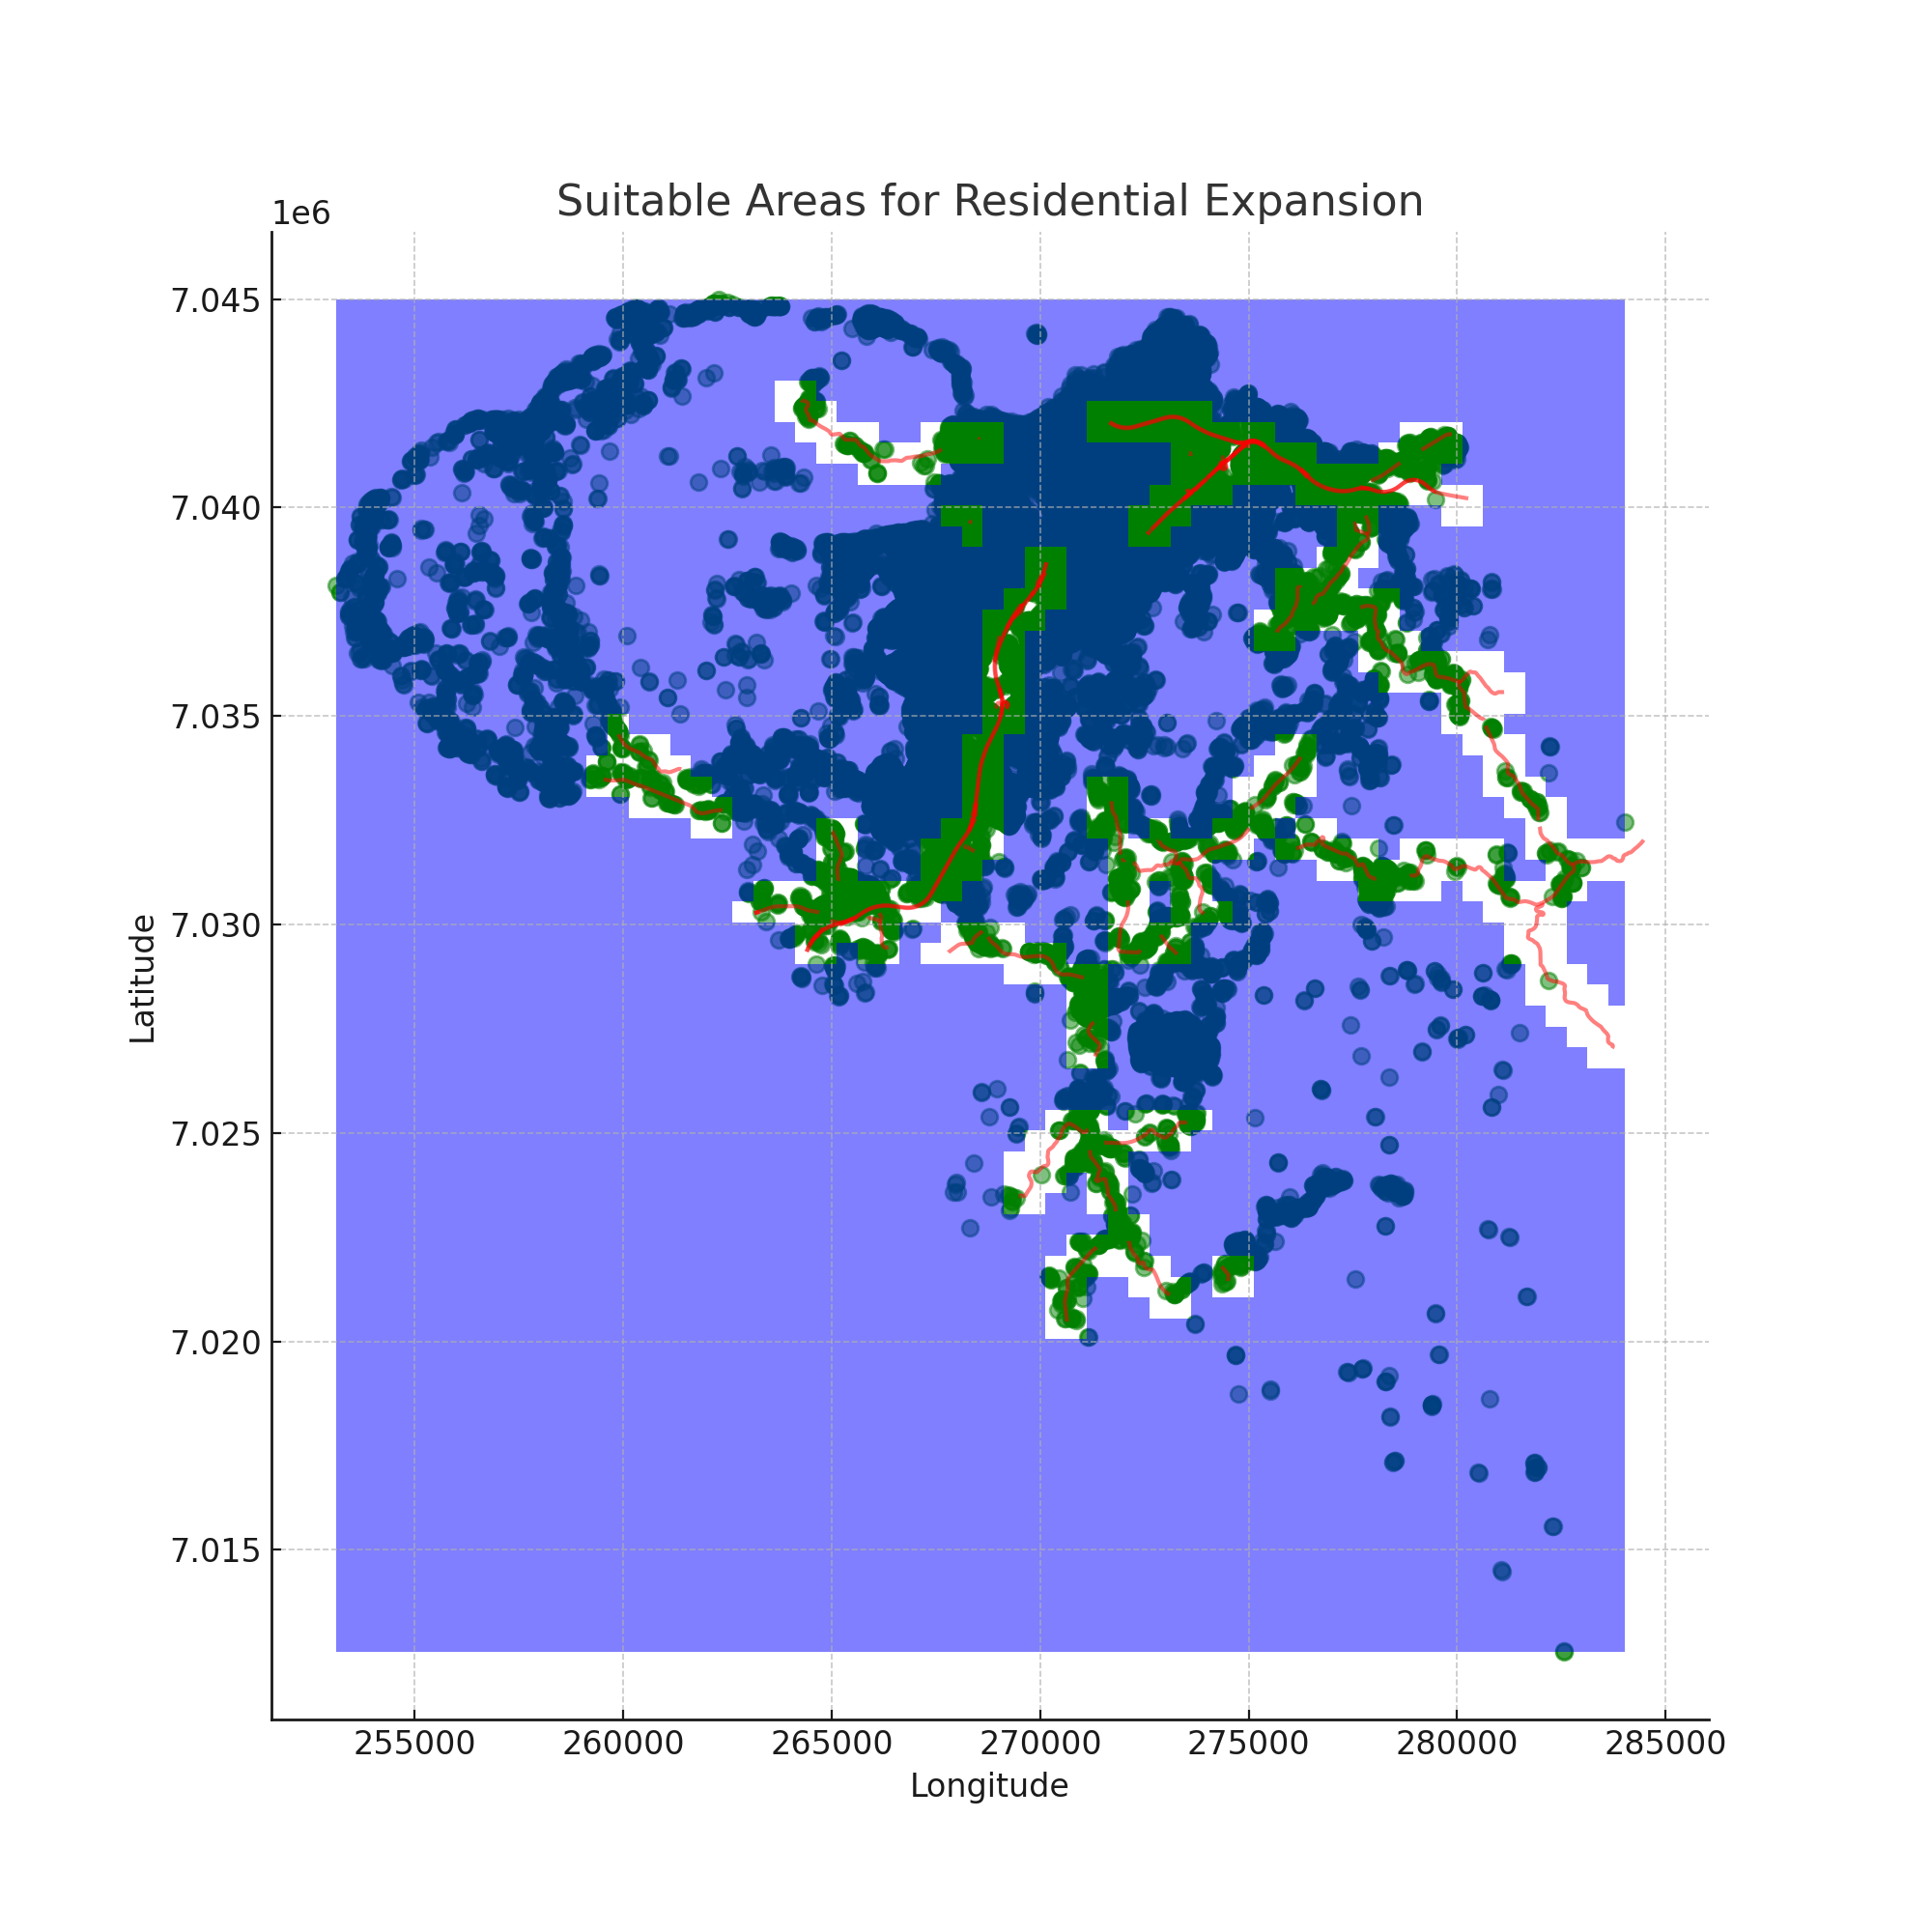
\includegraphics[width=\textwidth]{../figs/residential_expansion_areas_map.png}
    \caption{The result of ChatGPT when asked to \enquote{Find the area best suited for expansion to accommodate residential buildings}, using provided GeoJSON datasets. Potentially suitable areas for residential expansion  are depicted in blue.}
    \label{fig:planning-plot-from-geojson}
\end{figure}

Using the shapefile-formatted data, ChatGPT was able to produce a decent summary of the data, but the attribute names were cut off after about 10 characters. It was, however, able to produce a quite good visual representations of both datasets, colouring the roads differently by their speed limits and the buildings by their building type (see \autoref{fig:shapefile-visualization}). While it did manage to filter roads on speed limits, it could not calculate the mean location of the buildings. The \textit{Buffer + Intersect} and planning tasks again proved too complex.

\begin{figure}
    \centering
    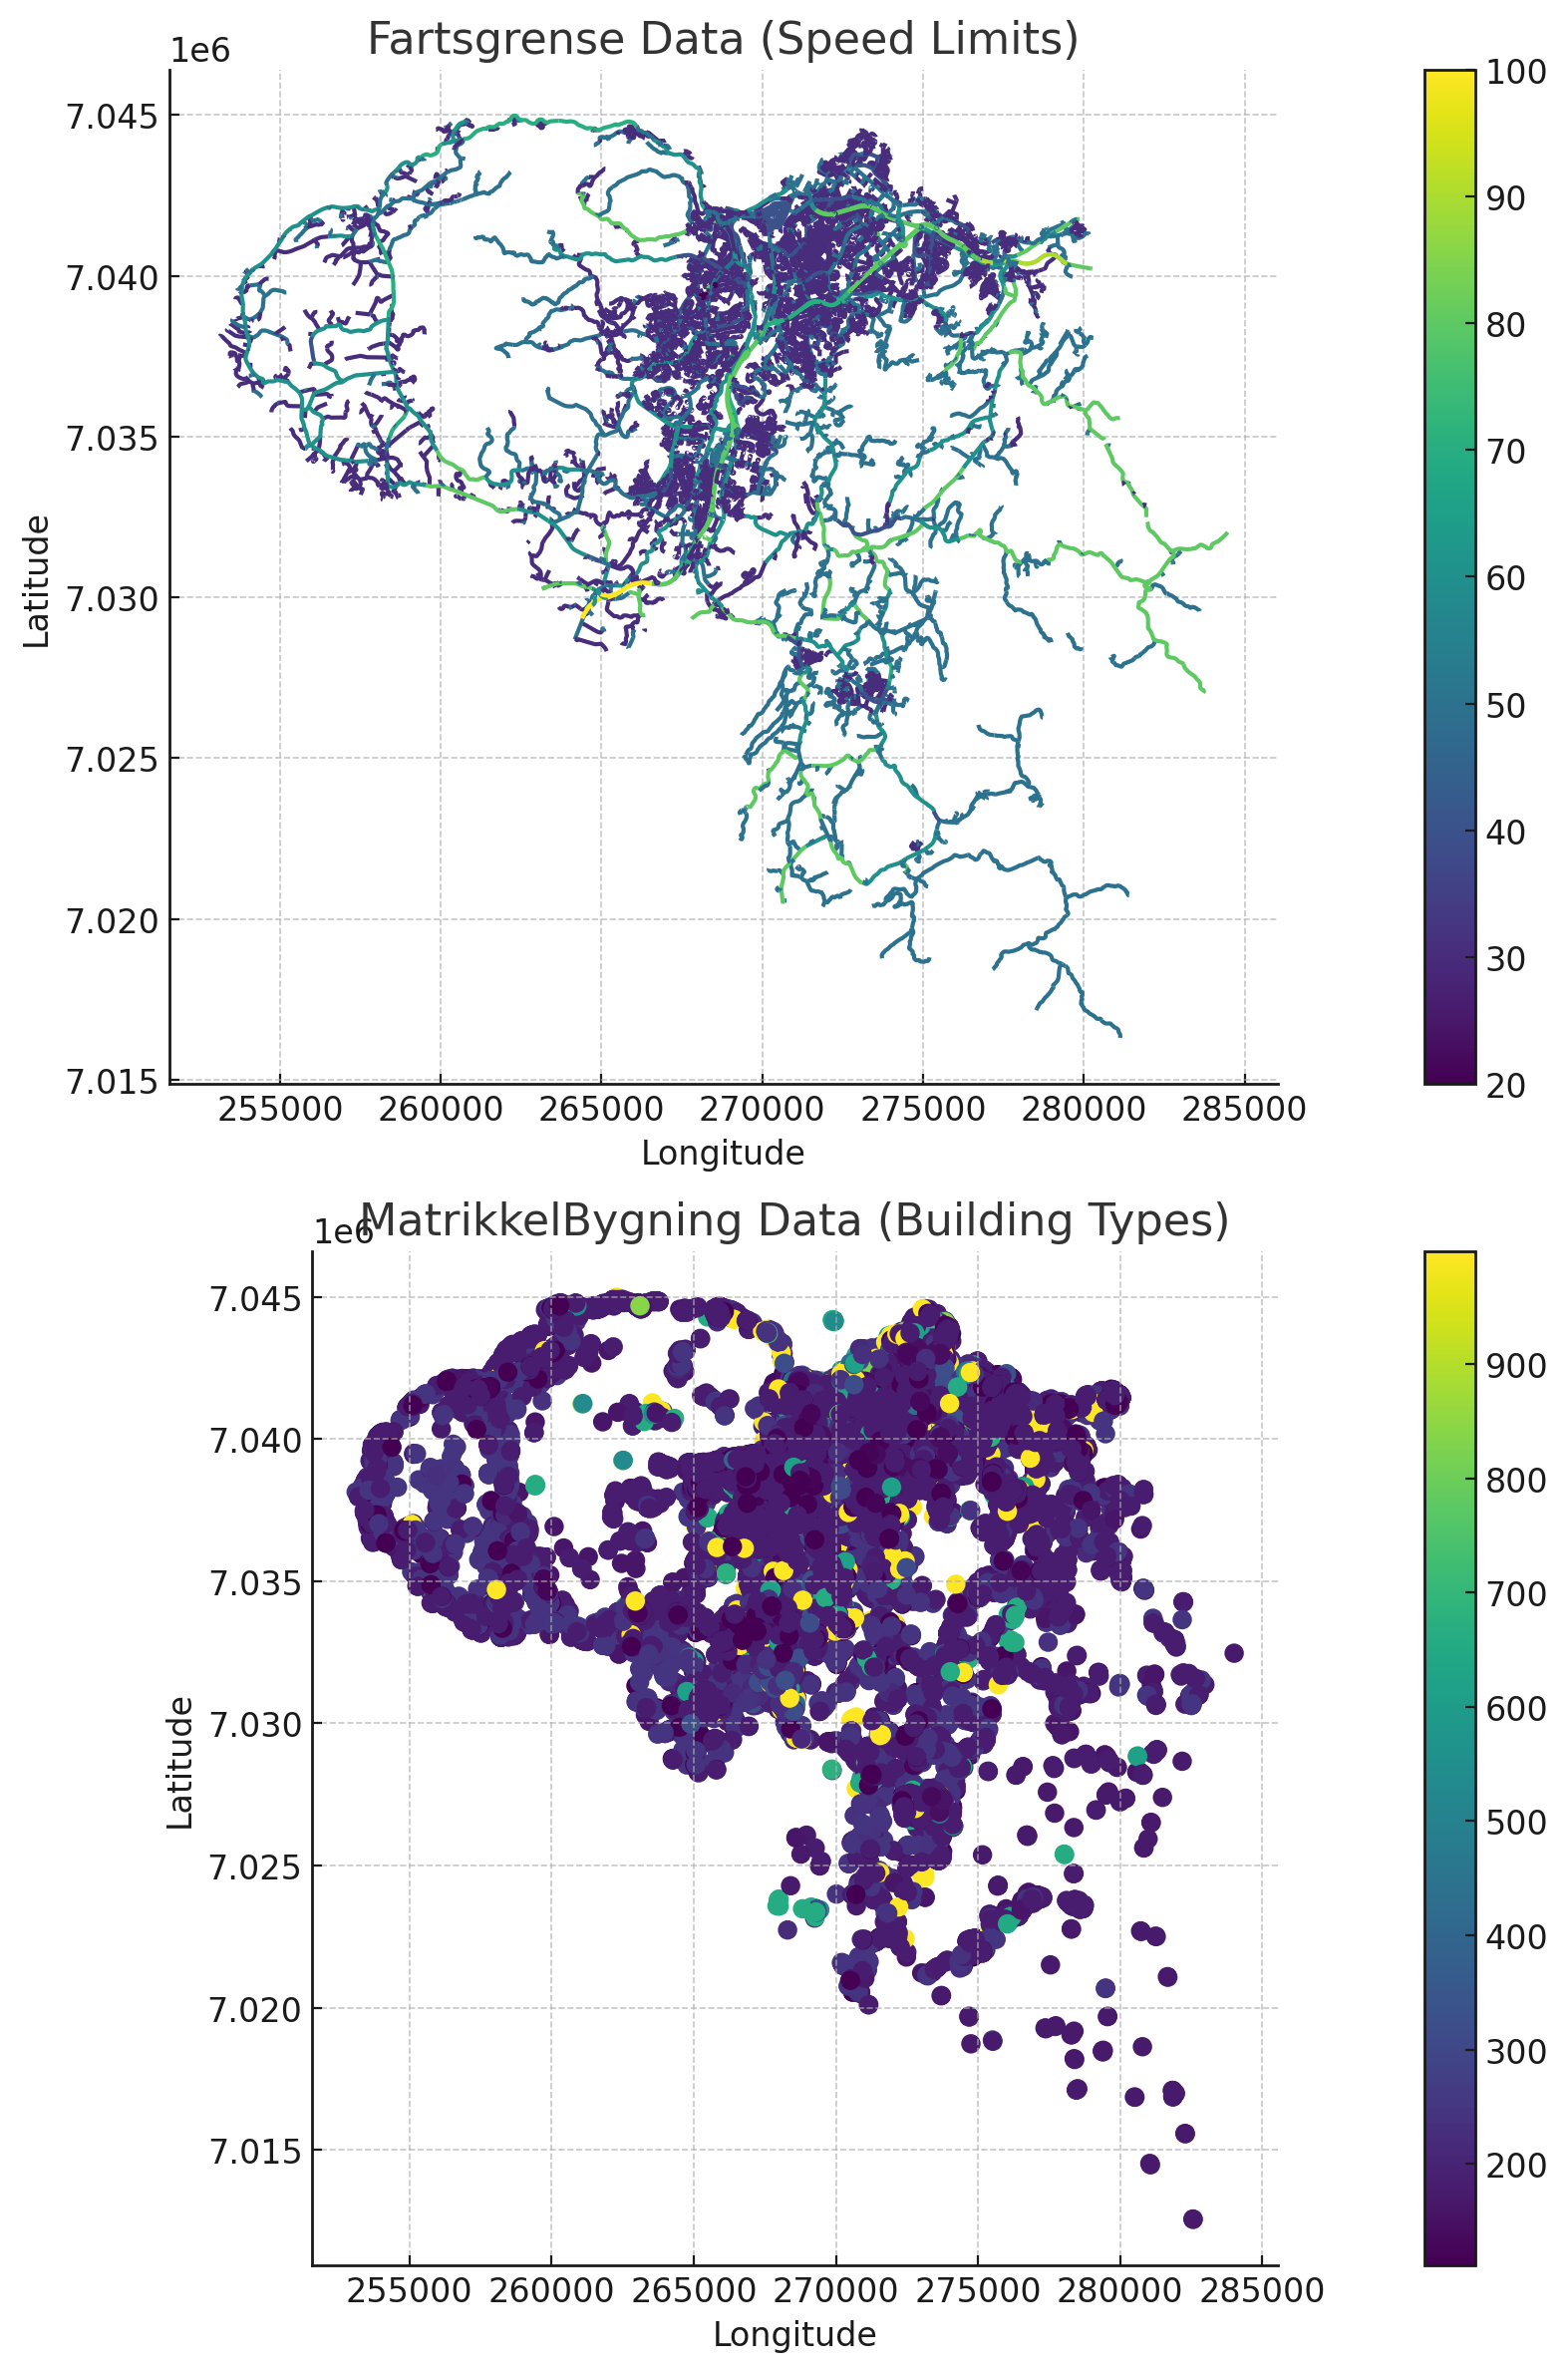
\includegraphics[width=0.7\textwidth]{../figs/shape_plot.png}
    \caption{Visual representations of shapefile datasets}
    \label{fig:shapefile-visualization}
\end{figure}

\subsection{Results for Experiment 2}\label{subsec:experiment-2-results}

\autoref{subfig:drammen-outline-file-upload} and \autoref{subfig:drammen-outline-api} show the results of providing ChatGPT-4 with the GeoJSON file for the outline of Drammen municipality using the file upload functionality, and supplying it with a URL to an \acrshort{acr:api} endpoint, respectively. While the Code Interpreter handled the direct file upload with ease, it struggled when provided with the URL to the corresponding web \acrshort{acr:api}. When provided with the URL, its first response was that \enquote{there was a problem with establishing a connection to the website}, after trying to process the request using Code Interpreter. When guided (twice) to try accessing the URL using its web browsing abilities instead, it was eventually able to read the data. In the subsequent prompt it was asked to provide a visual representation, but failed to do so successfully as \autoref{subfig:drammen-outline-api} shows. The reason for this was its decision to \enquote{truncate the dataset for brevity, using a subset of the full coordinate list} (see \autoref{lst:python-for-failed-drammen-outline}).

\begin{figure}
    \centering
    \begin{subfigure}{0.45\textwidth}
        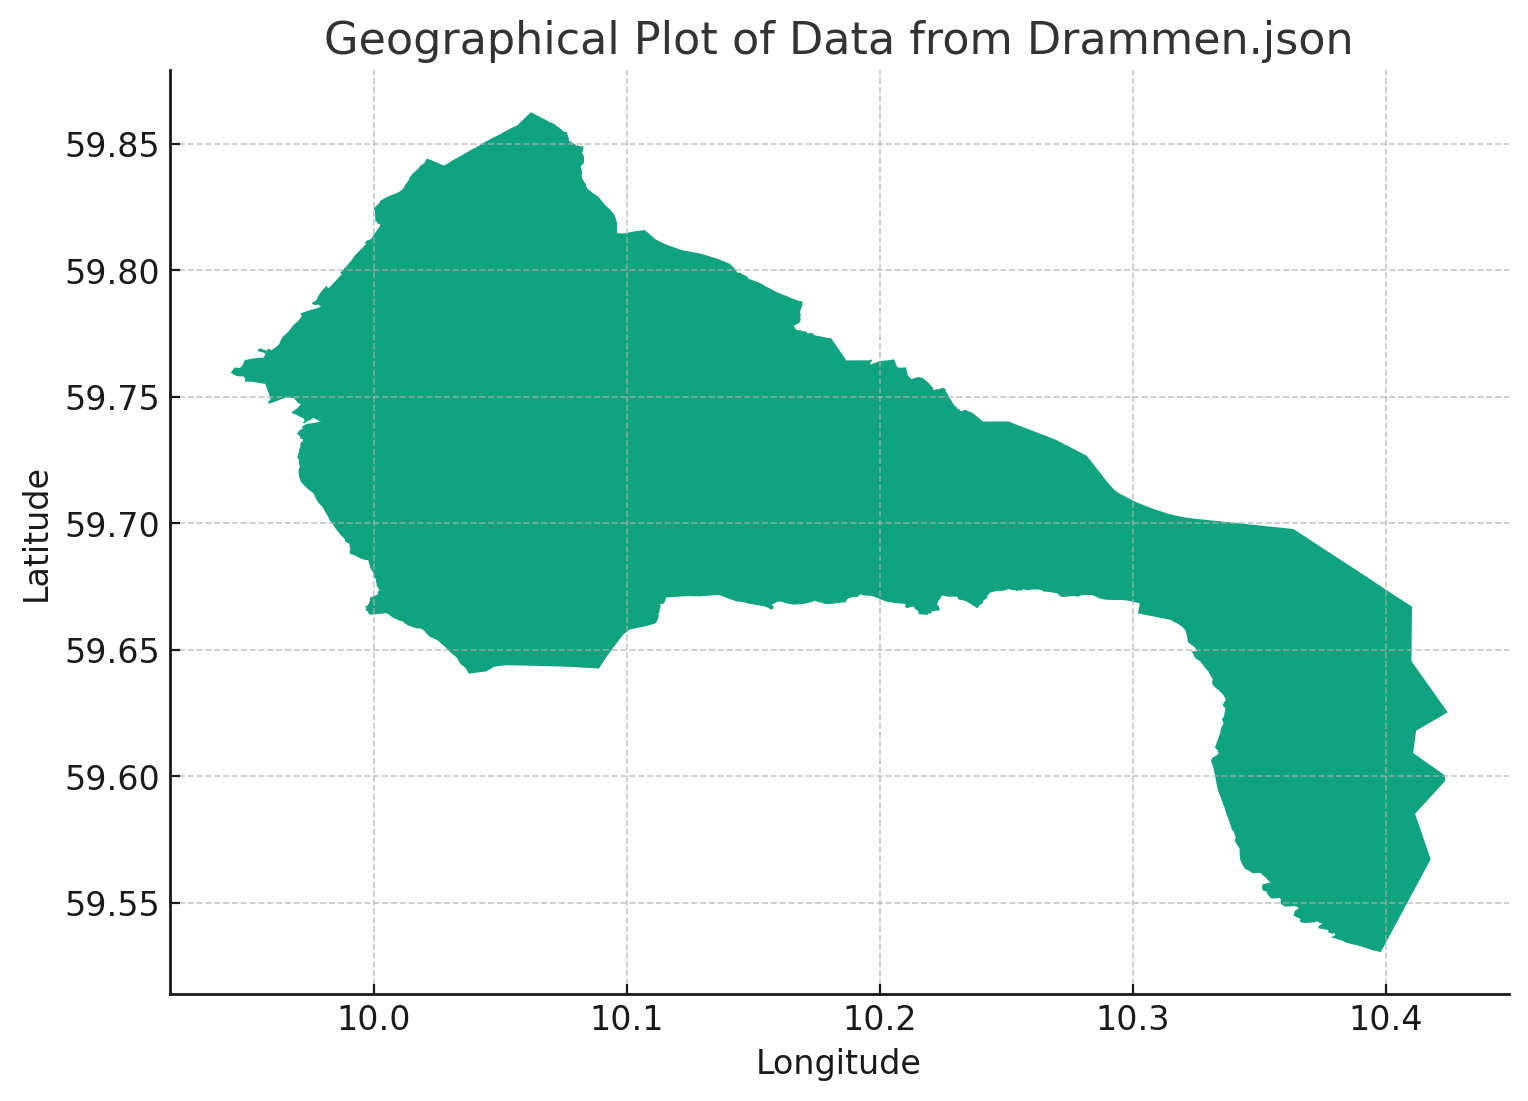
\includegraphics[width=\linewidth]{../figs/drammen_outline_file_upload.png}
        \caption{File upload}
        \label{subfig:drammen-outline-file-upload}
    \end{subfigure}
    \hfill
    \begin{subfigure}{0.45\textwidth}
        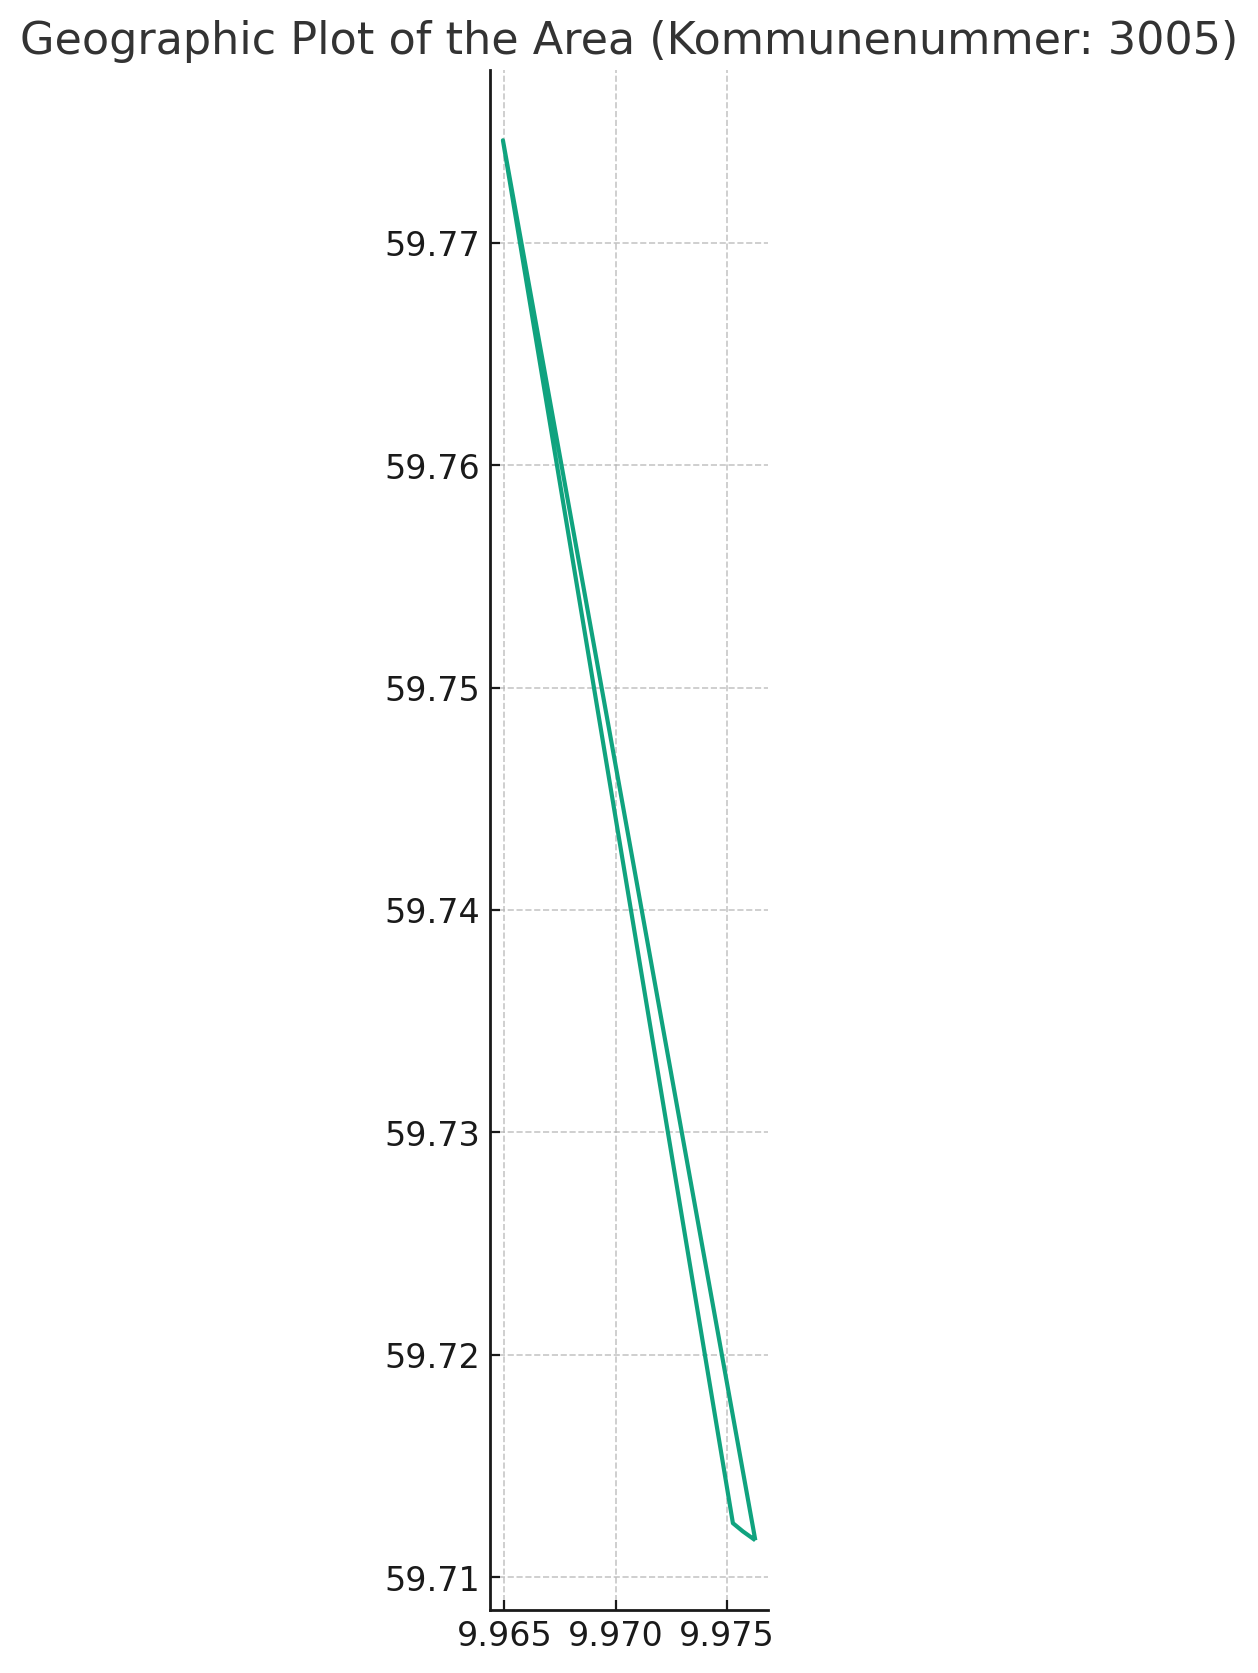
\includegraphics[width=\linewidth]{../figs/drammen_outline_api.png}
        \caption{Providing URL}
        \label{subfig:drammen-outline-api}
    \end{subfigure}
    \caption{Comparison of the resulting outlines/polygons of Drammen when using file upload (\subref{subfig:drammen-outline-file-upload}) and providing an URL to an API endpoint (\subref{subfig:drammen-outline-api}) with ChatGPT-4}
    \label{fig:file-upload-api-comparison}
\end{figure}

\begin{minipage}{\linewidth}
    \begin{lstlisting}[style=python, caption=ChatGPT code that truncates coordinates, label=lst:python-for-failed-drammen-outline]
# ...

# Extracted coordinates from the JSON data
coordinates = [
    [[9.976278541184014, 59.71166107645171], [9.975715936016496, 59.71206324390201], [9.975270250797282, 59.71243147807226], 
    # ... Truncated for brevity, using a subset of the full coordinate list
    [9.964929990238785, 59.774609947672644]]
]

# ...
\end{lstlisting}
\end{minipage}

\subsection{Results for Experiment 3}\label{subsec:experiment-3-results}

The setup described in \autoref{subsec:ex-3-setup}, which allows the \texttt{AgentExecutor} from LangChain to autonomously make arbitrary calls to the \texttt{gpt-4-1106-preview} model, successfully called the two functions in the correct order and with the appropriate arguments. It first decided to call \texttt{make\_http\_request(url: str, save\_file\_name: str)} using the provided URL to the \acrshort{acr:api} endpoint and \enquote{kommuner.geojson} as function arguments. As expected, the function call resulted in a GeoJSON file called \enquote{kommuner.geojson} being stored at \texttt{/tmp/kommuner.geojson}. The file name is likely derived from the URL it was provided with, as it did not have any knowledge about the file contents at the time of saving. The \texttt{AgentExecutor}---powered by \acrshort{acr:gpt}-4---then correctly decided to call \texttt{plot\_geojson(geojson\_path: str)} using \enquote{kommuner.geojson} as the function argument. This resulted in \autoref{fig:drammen-plot-langchain}, which correctly show the outline of Drammen municipality. Since this last function returns the string \enquote{File plotted successfully} after having plotted the file contents, the \texttt{AgentExecutor} correctly decided to terminate the chain. The notebook used for the experiment is available on the project GitHub repository\footnote{\url{https://github.com/oskarhlm/prosjektoppgave/blob/main/src/python/examples/drammen_ogc_test/drammen_ogc_test.ipynb}}.

\begin{figure}
    \centering
    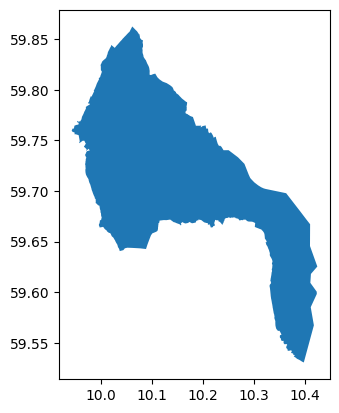
\includegraphics[width=0.4\textwidth]{../figs/drammen_plot_langchain.png}
    \caption{Outline of Drammen using LangChain and OpenAI Functions}
    \label{fig:drammen-plot-langchain}
\end{figure}

\glsresetall
